\documentclass{article}
\usepackage[utf8]{inputenc}
\usepackage{hyperref}
\usepackage[letterpaper, portrait, margin=1in]{geometry}
\usepackage{enumitem}
\usepackage{amsmath}
\usepackage{booktabs}
\usepackage{graphicx}
\usepackage{float}


\usepackage{hyperref}
\hypersetup{
colorlinks=true,
    linkcolor=black,
    filecolor=black,      
    urlcolor=blue,
    citecolor=black,
}
\usepackage{natbib}

\usepackage{titlesec}
  
\title{Homework 8}
\author{Ioanna Maria Spyrou}
\date{Spring semester 2021}
  
\begin{document}
  
\maketitle


1. The design should be a sharp RD. Sharp RD is the appropriate design because treatment status is a deterministic and discontinuous function $D_i$ of length which takes values 0 or 1 depending on the cutoff. We know that 225 inches is the cutoff. The assignment mechanism is a deterministic function of length because once we know length we know whether $D_i$ will be 0 or 1. Treatment is a discontinuous function of length because no matter how close length gets to 225 inches, treatment is unchanged until length equals 225.  \\

2. 
\begin{figure}[H]
\centering
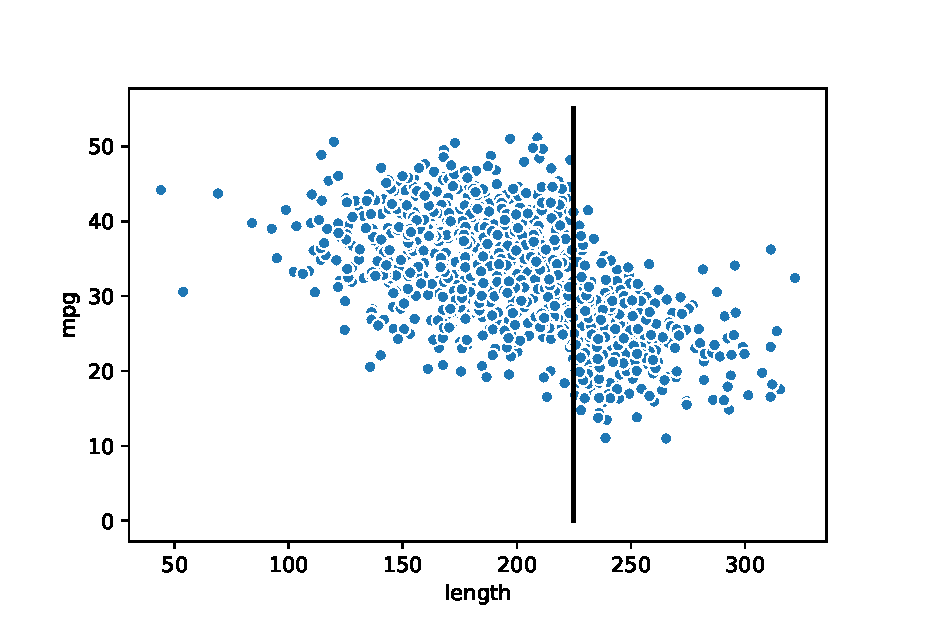
\includegraphics[scale = 0.7]{figure1.eps}
\caption{Scatterplot of mpg and length with cutoff line.}
\end{figure}

It is clear from figure 1 that at 225 inches there is discontinuity.\\

3.See figure 2.
\begin{figure}[H]
\centering
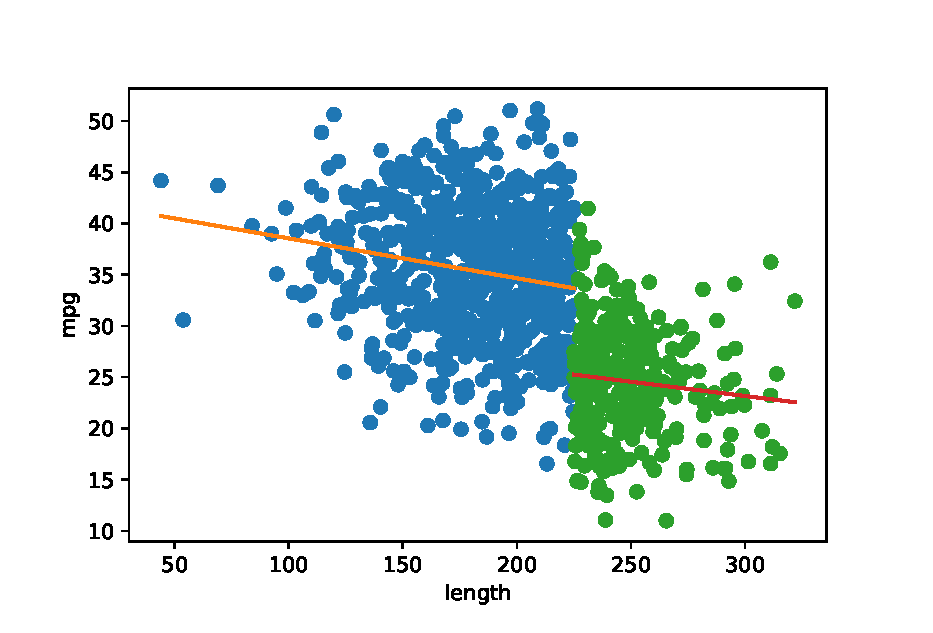
\includegraphics[scale = 0.7]{figure2.eps}
\caption{First-order polynomial over scatterplot.}
\end{figure} 

The impact of the policy on fuel efficiency around the cutoff is 8.429.\\

4.See figure 3.
\begin{figure}[h]
    \centering
    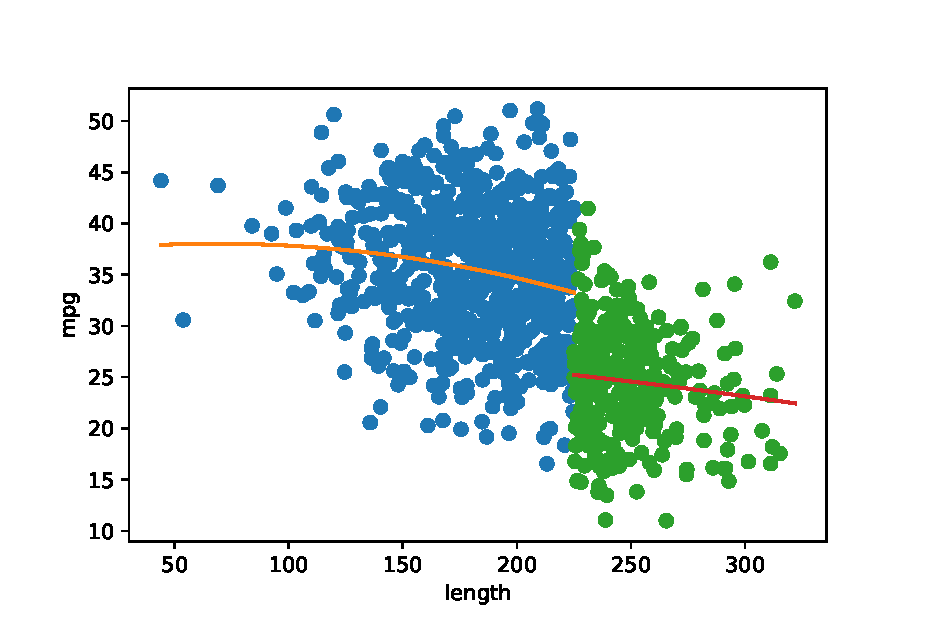
\includegraphics[scale = 0.7]{figure3.eps}
    \caption{Second-order polynomial over scatterplot.}
\end{figure}

 The impact of the policy on fuel efficiency around the cutoff is 8.048.\\

5. see figure 4.
\begin{figure}[H]
    \centering
    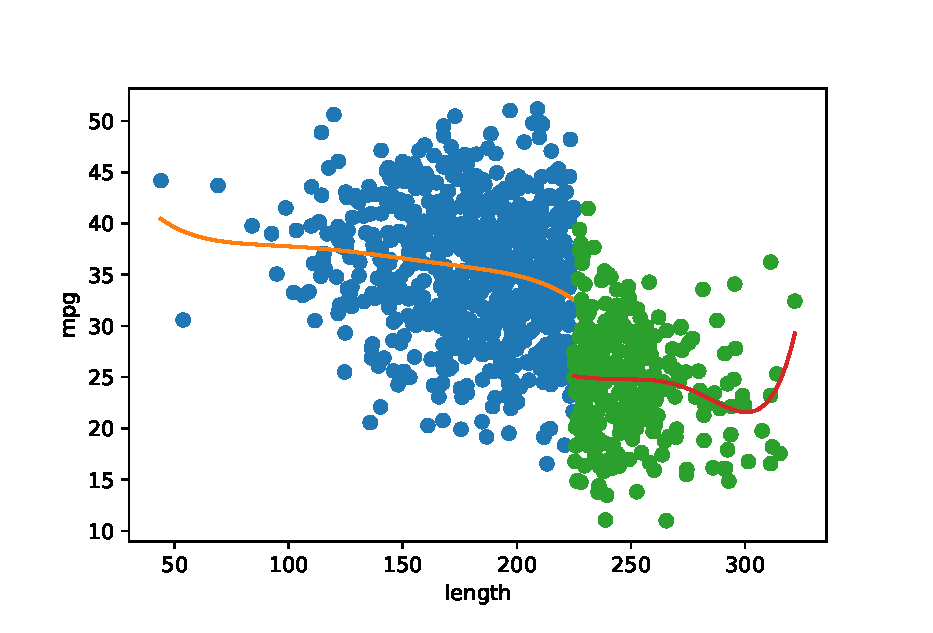
\includegraphics[scale = 0.7]{figure4.eps}
    \caption{Fifth-order polynomial over scatterplot.}
\end{figure}

The impact of the policy on fuel efficiency around the cutoff is 7.438.\\

6.We can see that the impact of the policy on fuel efficiency is similar in all three cases. According to Gelman and Inbems (2014) using high-order polynomials can be misleading, so local linear or quadratic are preferred. Moreover, high-order polynomials may assign too much weight to observations far away from RD cutoff. So fifth-order polynomial is not appropriate.The seminal work of Hahn, Todd and Van der Klaauw (2001) correctly states that the local linear estimator has an asymptotically smaller bias than the kernel regression estimator, but according to Porter (2003), by the same argument, any higher-order polynomial will have an even smaller asymptotic bias than the local linear. The used polynomial for the first stage is second-order polynomial. See table \ref{tab:coeftable}:

\begin{table}[h]
    \centering
    \begin{tabular}{lll}
\toprule
{} &        (a) &       (b) \\
\midrule
Firmsize        &    9714.72 &      9.35 \\
                &  (3961.76) &   (25.27) \\
Treatment group &     130.30 &   3676.38 \\
                &   (355.08) &  (355.47) \\
Shrimp          &       1.54 &      1.54 \\
                &     (0.06) &    (0.06) \\
Salmon          &      -0.41 &     -0.41 \\
                &     (0.26) &    (0.26) \\
Treated         &   -8110.31 &  -8110.31 \\
                &   (611.32) &  (611.32) \\
\bottomrule
\end{tabular}

    \caption{Second-stage regression coefficients table with standard errors.}
    \label{tab:coeftable}
\end{table}
\\
Based on the F-statistic for significance of the instrument in the first-stage, which is 665.1 and exceeds 10, it is a valid instrument.



\end{document}